%Arrumar as citações e tentar ajustar as marcações em vermelho

\chapter{Metodologia}

Neste capítulo será detalhado os três módulos propostos na figura \ref{fig:proposta}: Condições Iniciais, Treinamento e Geração de Sequências. 

\section{Condições iniciais}
O objetivo do primeiro módulo (figura \ref{fig:cond_iniciais}) é obter a sequência e o erro inicial. 
A primeira é obtida ao se passar a estrutura alvo como entrada do \textit{ProteinMPNN}.
Já o erro inicial é definido pela seguinte expressão:
 
\begin{equation}
    Er_{0} = 1 - TMScore(E_{FIX}, E_{ini})
\end{equation}

\noindent
Onde $E_{FIX}$ é a estrutura alvo, i.e, a estrutura do fator IX de coagulação e $E_{ini}$ é a estrutura vinculada a sequência inicial, 
predita pelo \textit{ESMFold} - descrito em \ref{subsection:structure_pred}. 
O \textit{TMScore} consiste em uma medida de similariedade entre estruturas, detalhada em \ref{subsection:tmscore}

\begin{figure}[H]
  \centering
  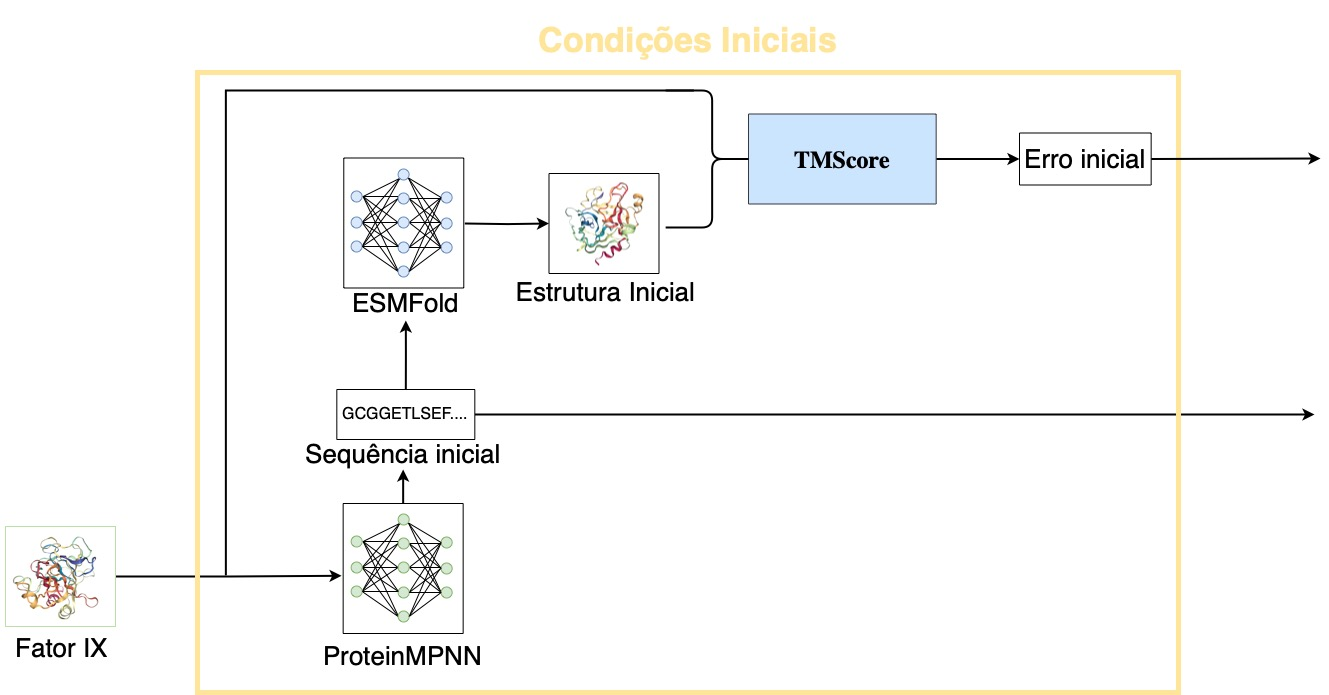
\includegraphics[width=.8\textwidth]{figuras/metodologia-Initial_cond.jpg}
  \caption{Obtenção das condições iniciais}
  \label{fig:cond_iniciais}
\end{figure}

\section{Treinamento}
%iterações entre Agente e Ambiente ok
%Agente é PPO ok
%Acao é mutação ok 
%Imagem da mutação ok 
%Ambiente de aprendizado é modelado por um MDP e é definido quem sao os estados, acoes e  recompensas. É tambem definido a função de transição entre estados (step) e função de reset
O módulo de Treinamento foi construído em duas etapas: Estágios I e II, detalhados em \ref{subsection:stage1} e \ref{subsection:stage2} respectivamente.
Para ambos os estágios, o treinamento se dá através de interações entre dois componentes: O Ambiente de aprendizado e o Agente. 

\subsection{Ambiente de aprendizado}
O ambiente de aprendizado é modelado como um MDP e, portanto, é responsável por definir o espaço de ações, o espaço de estados, a função de transição entre estados dado uma ação e a função de recompensa.  

\subsubsection{Espaço de ações}

Definimos uma ação como um vetor bi-dimensional composto pelo índice $p$ de uma posição na sequência e um aminoácido $r$. 
A ação será utilizada para realizar uma mutação na proteína, inserindo o $r$ na posição $p$. 
De modo a incentivar o Agente a explorar diferentes ações, 
definimos, para cada iteração, um conjunto de posições e aminoácidos válidos: $P_{val}$ e $R_{val}$ respectivamente. 
$P_{val}$ é composto por todas as possíveis posições na sequência, com exceção das posições previamente selecionadas dentro do mesmo episódio. 
Definimos $R_{val}$ sendo igual aos 20 possíveis aminoácidos, com exceção dos aminoácidos que foram selecionados mais de 7 vezes no mesmo episódio. 
Desta forma, o espaço de ações, para cada iteração $i$, é definido por:

\begin{equation}
A_{i} = \left\{(p, r) | p \in P_{val_{i}} , r \in R_{val_{i}} \right\}
\end{equation}
  

\subsubsection{Espaço de estados}
Definimos o espaço de estados como o conjunto de todas as possíveis sequências de $n$ aminoácidos, onde $n$ é o tamanho da sequência inicial:

\begin{equation}
S = \left\{(r_{1}, r_{2}, r_{3}, ..., r_{n}) | r_{i} \in R_{encoded} \forall i \in [1,n] \right\}
\end{equation}

Onde $R_{encoded}$ é o conjunto dos 20 possíveis aminoácidos, 
cada um representado por um vetor codificado pelo \textit{Encoder}. 
O \textit{Encoder} consiste em um dicionário que mapeia cada aminoácido para 
uma representação vetorial que conserva as distâncias entre cada par de aminoácidos estabelecidas por \cite{aminodist}.
Este mapeamento foi construído através de um MDS utilizando 21 dimensões. 

\begin{figure}[H]
  \centering
  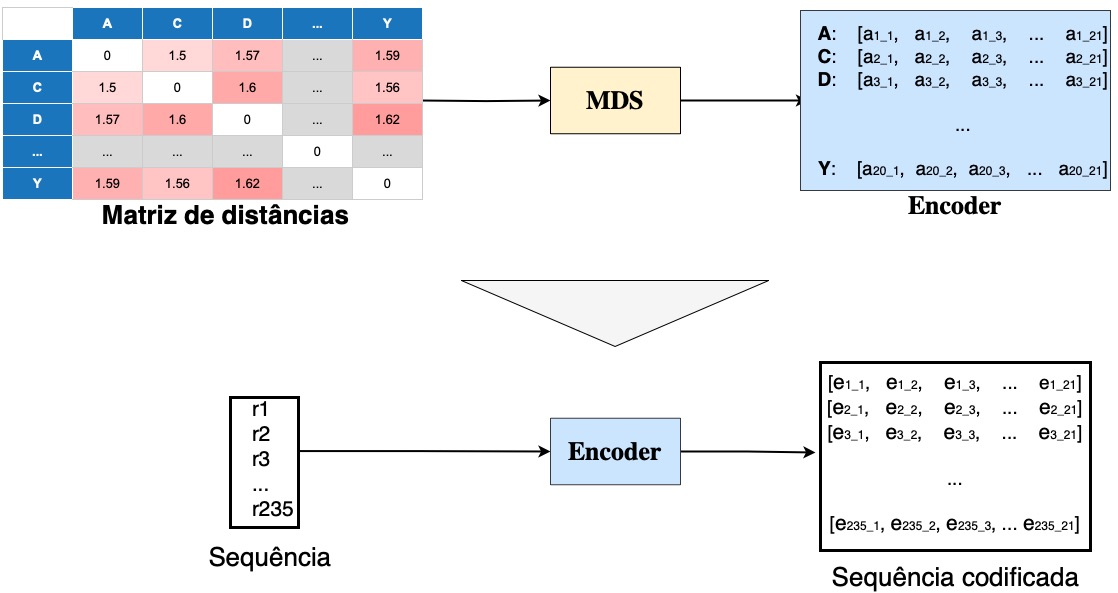
\includegraphics[width=.8\textwidth]{figuras/metodologia-encoder.jpg}
  \caption{Construção e uso do \textit{Encoder}. }
  \label{fig:encoder}
\end{figure}

Para escolher a quantidade de dimensões a se utilizar no MDS, definimos o ponto a partir do qual a curva entre \textit{Stress} e dimensionalidade 
tende a se aproximar assintóticamente do eixo x do plano cartesiano. Este ponto, conforme a figura \ref{fig:best_dim}, é o que possui 21 dimensões. 

\begin{figure}[H]
  \centering
  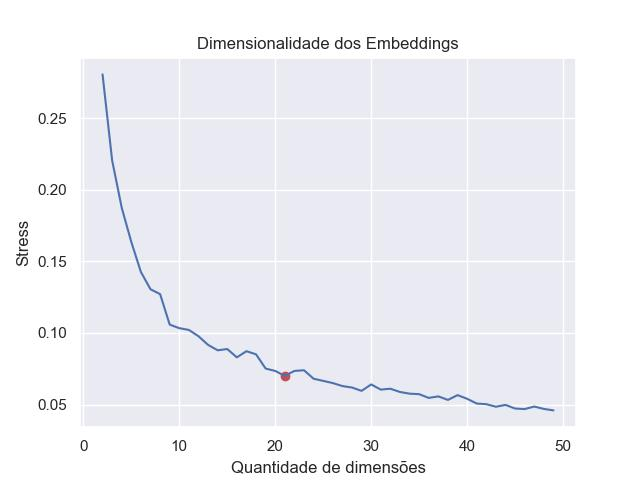
\includegraphics[width=.8\textwidth]{figuras/best_dim.jpg}
  \caption{Escolha da dimensionalidade dos Embeddings}
  \label{fig:best_dim}
\end{figure}



\subsubsection{Função de transição de estados}
A função de transição de estados é caracterizada pela geração de uma nova sequência, 
resultante da mutação definida pelo Agente. 
Em outras palavras, é uma função que tem como entrada uma ação e o estado atual e como saída o estado resultante da transição. 

\begin{figure}[H]
  \centering
  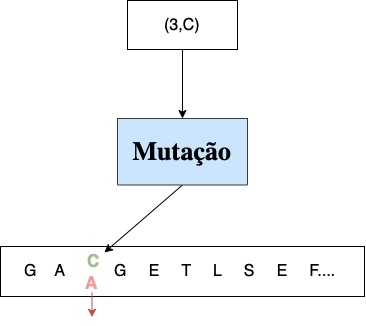
\includegraphics[width=.8\textwidth]{figuras/metodologia-Mutation.jpg}
  \caption{Exemplo de mutação. O aminoácido A na posição 3 está sendo substituído pelo o aminoácido C}
  \label{fig:mutacao}
\end{figure}

\subsubsection{Função de recompensa}
Já a função de recompensa calcula a qualidade da ação selecionada pelo Agente. 
Nas seções \ref{subsection:stage1} e \ref{subsection:stage2} especificamos a função de recompensa de cada estágio de treinamento.


\subsection{Agente}
\label{subsection:Agente}
O Agente é modelado por uma rede neural, batizada de \textit{GenSeq}, cujos parâmetros são otimizados através da técnica \textit{Proximal Policy Optimization} (PPO), 
sendo responsável por decidir qual a melhor mutação a se fazer, dada a sequência de entrada. Em outras palavras, o Agente deve escolher,
dentro do espaço de ações, a ação que maximiza a recompensa acumulada.
Os hiperparâmetros utilizados no Agente são apresentados na tabela a seguir. 

\begin{table}[H]
\centering
\vspace{0.5cm}
\begin{tabular}{r|lr}
Hiperparâmetro & Valor \\ 
\hline                               
Número de camadas escodidas & 2 \\
Número de neurônios por camada escondida & 64 \\
Função de ativação & tangente hiperbólica \\
Otimizador & Adam \\
Taxa de aprendizagem & 3e-4 \\
Número de épocas & 10 \\
Fator de desconto ($\gamma$) & 0.99 \\
\end{tabular}
\caption{Hiperparâmetros do PPO}
\end{table}

Após ser processada pelo \textit{Encoder}, a sequência passa pela camada de entrada do \textit{GenSeq} e 
segue para duas camadas escondidas de 64 dimensões cada. 
A camada de saída, por sua vez, possui 255 unidades, organizadas em duas partes:

\begin{enumerate}
  \item As primeiras 235 unidades da camadas estão associadas ao primeiro atributo da ação: A posição $p$ da sequência de entrada
  que deve sofrer mutação. A posição predita pelo Agente corresponde ao índice da unidade de saída com maior valor entre as 235 primeiras. 
  \item Já as 20 últimas unidades de saída estão associadas ao segundo atributo da ação: O índice do aminoácido $r$ que o Agente sugere inserir na posição $p$.
  Este valor corresponde ao índice da unidade de saída com maior valor entre as 20 últimas unidades, subtraído de 235.
\end{enumerate}

Por exemplo, suponha que, entre as 235 primeiras unidades, a de maior valor é a terceira, e que, entre as 20 útltimas, o maior valor esteja na unidade 240. 
Nesse caso, a ação sugerida pelo Agente é fazer uma mutação na posição 3, inserindo o aminoácido de índice 5.

\begin{figure}[H]
  \centering
  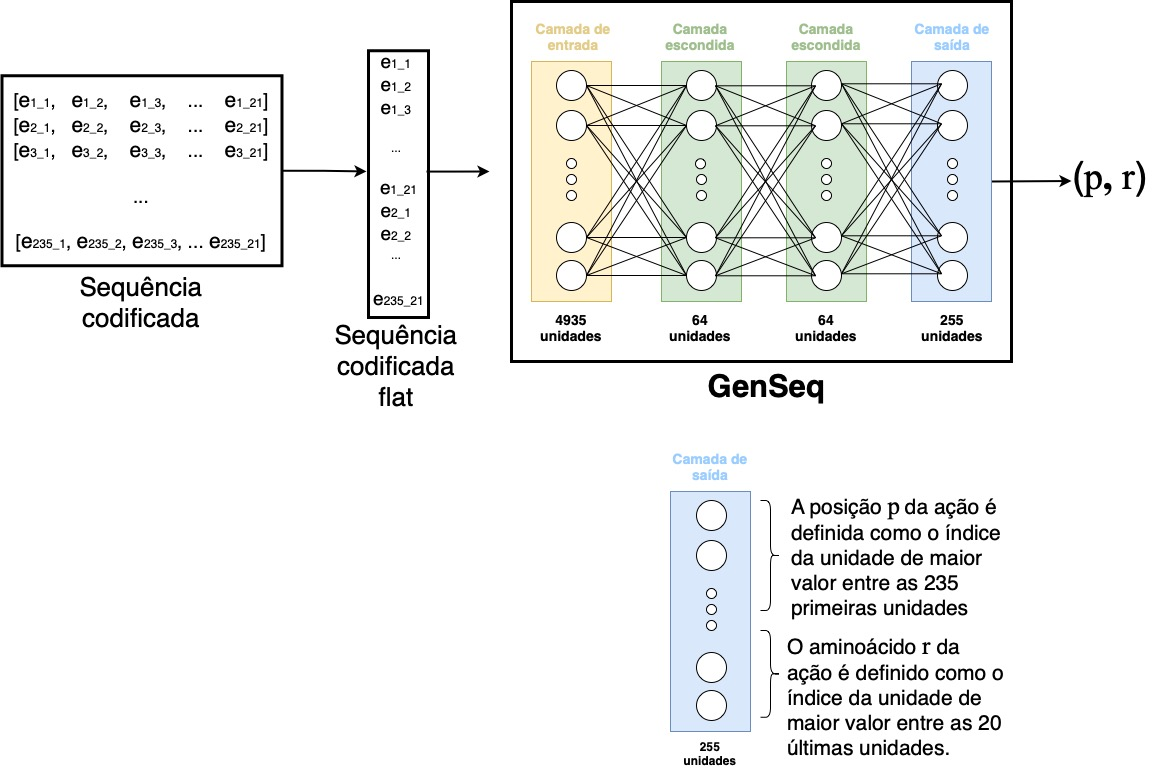
\includegraphics[width=.8\textwidth]{figuras/metodologia-NN_arch_actor.jpg}
  \caption{Arquitetura da rede neural do Agente (\textit{GenSeq})}
  \label{fig:actor_arch}
\end{figure}


\subsection{Treinamento - Estágio I}
\label{subsection:stage1}
%Definição de episodio 
%Vitoria ou derrota no episodio
%Numero de steps total e por episodio

Tendo em vista o vasto número de ações possíveis, 
desenvolvemos o Estágio I de treinamento com o objetivo de estimular o Agente a encontrar um subespaço menor de ações para atuar.
Para isso, atribuímos recompensas negativas (ou penalizações) para ações em posições da sequência cujo o \textit{Conservation Score} é alto,
bem como penalizamos ações onde o aminoácido substituído é muito diferente do que fora inserido. 
Neste sentido, definimos a seguinte função de recompensa:

\begin{equation}
    R_{I} = -(CS(p) + AminoDist(r, r_{prev}))
\end{equation}

\noindent
Onde $p$ e $r$ são a posição e o aminoácido selecionados pelo Agente, respectivamente. O $r_{prev}$ é o aminoácido que estava na posição $p$ antes da mutação. 
$CS(p)$ é o \textit{Conservation Score} normalizado da posição $p$ e $AminoDist(r, r_{prev})$ é a medida de similariedade entre os aminoácidos $r$ e $r_{prev}$. 

Neste sentido, o primeiro estágio de treinamento consiste do seguinte procedimento:

\begin{enumerate}
  \item Os pesos do \textit{GenSeq} são inicializados aleatóriamente.
  \item Inicializa o episódio com a sequência inicial e com $P_{val}$ sendo todas as posições da sequência e $R_{val}$ sendo todos os 20 aminoácidos 
  \item A sequência atual é codificada pelo \textit{Encoder}.
  \item \textit{GenSeq} estima a melhor ação $(p,r)$ baseado na sequência codificada. 
  \item A sequência atual é modificada ao inserir $r$ na posição $p$.
  \item Baseado em $(p,r)$ e $r_{prev}$, é calculado $R_{I}$.
  \item $p$ é removido de $P_{val}$ e se a quantidade de vezes que $r$ foi utilizado pelo \textit{GenSeq} é maior ou igual a 7, então $r$ é retirado de $R_{val}$.
  \item Se a iteração atual é igual ao tamanho do \textit{batch}, então \textit{GenSeq} atualiza seus pesos baseado nos valores obtidos de $R_{I}$ utilizando o \textit{PPO}
  \item Se foi atingido o máximo de mutações por episódio, então o episódio é finalziado.
  \item Repete a partir do item 2 até atingir o número máximo de iterações. 
\end{enumerate}


\begin{figure}[H]
  \centering
  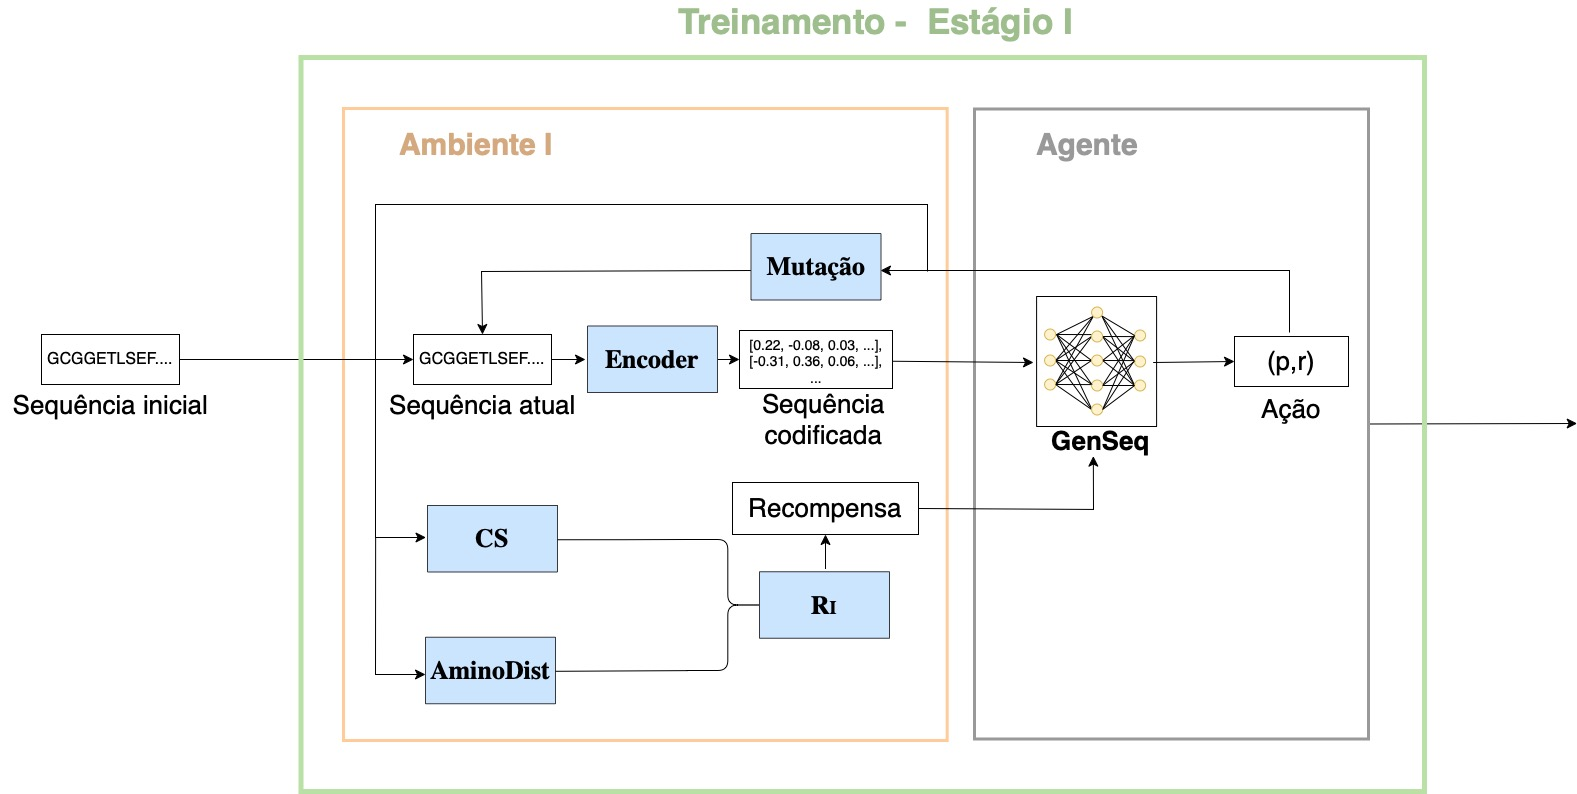
\includegraphics[width=.8\textwidth]{figuras/metodologia-Pre-Training.jpg}
  \caption{Primeiro estágio de treinamento}
\end{figure}

Neste estágio, o Agente foi treinado com um total de 2 milhões de iterações, podendo executar até 100 mutações por episódio.
\begin{table}[H]
  \centering
  \vspace{0.5cm}
  \begin{tabular}{r|lr}
  Parâmetro & Valor \\ 
  \hline                               % para uma linha horizontal
  Número máximo de mutações por episódio & 100 \\
  Número de iterações & 2.000.000 \\
  Tamanho do \textit{batch} & 200 \\
  \end{tabular}
  \caption{Parâmetros preliminares}
  \end{table}

  Após finalizado o primeiro estágio, comparamos o desempenho do Agente com o desempenho de uma política que define ações aleatoriamente, onde observamos
  que a mediana da distribuição de recompensas do Agente é consideravelmente superior ao do Agente aleatório. 

  \begin{figure}[H]
    \centering
    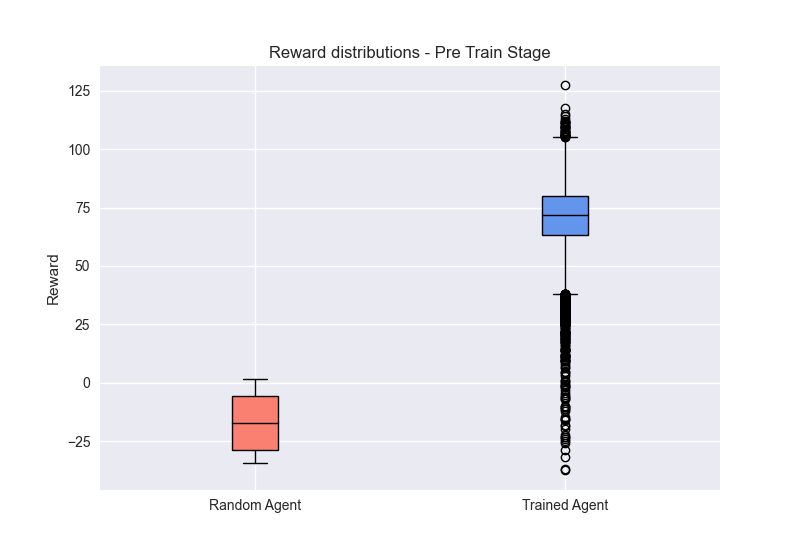
\includegraphics[width=.8\linewidth]{figuras/plot_box_pre_train_reward.jpg}  
    \caption{Comparação do Agente pré treinado com um Agente aleatório}
    \label{fig:box-pre-train}
  \end{figure}

Observa-se que o Agente atingiu um platô de recompensas no ambiente I com cerca de 2500 episódios, como ilustrado em 
\ref{fig:rew_per_ep_pretrain}.

  \begin{figure}[H]
    \centering
    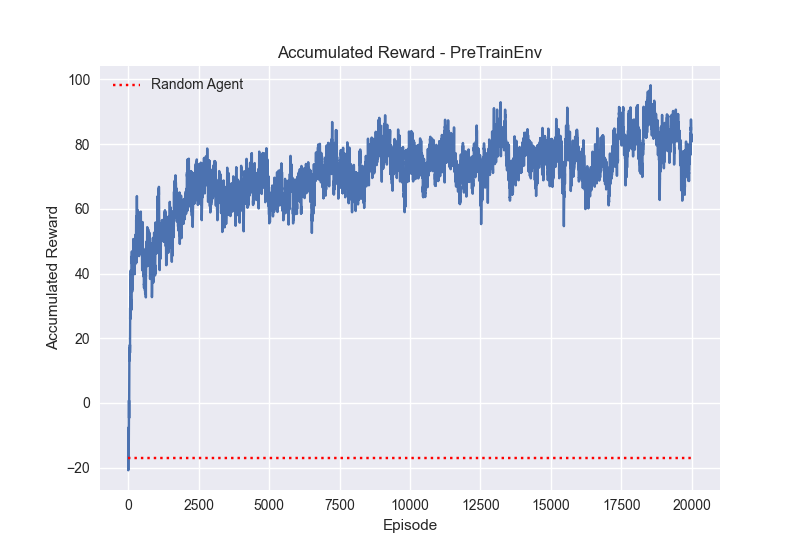
\includegraphics[width=.8\linewidth]{figuras/plot_pre_train_reward.jpg}    
    \caption{Média móvel das recompensas por episódio - treino}
    \label{fig:rew_per_ep_pretrain}
  \end{figure}


\subsection{Treinamento - Estágio II}
\label{subsection:stage2}
%Função do reward
%Numero de steps total e por episodio
%Vitoria ou derrota no episodio
O objetivo do segundo estágio de treinamento é fazer com que o agente pré treinado aprenda a escolher ações que maximizem o \textit{TM-Score} entre a estrutura gerada e a alvo, 
i.e, minimizem o erro $1-TMScore$.
Para isto, definimos a função de recompensa como a soma de 3 termos: 

\begin{equation}
    R_{II} = -aEr_{i} + b(Er_{0} - Er_{i}) + c(Er_{i-1} - Er_{i})
\end{equation}

\noindent
Onde $Er_{i}$ e $Er_{i-1}$ são os erros da iteração i e i-1 respectivamente, e $a, b$ e $c$ são constantes. 
O primeiro termo, $-aEr_{i}$, é a penalização pelo erro atual.
O segundo determina uma penalização se o erro atual for maior que o inicial e uma recompensa caso contrário.
Análogamente, o terceiro termo penaliza se o erro atual for maior que o anterior e recompensa se for menor.
Como o objetivo principal é encontrar sequências com erro menores que o inicial, atribuímos um peso maior ao segundo termo, i.e, $b>a$ e $b>c$.
Além disso, consideramos $c>a$ para valorizar reduções do erro ao longo do episódio.  

Introduzimos o conceito de vitória e derrota a cada episódio. 
Consideramos vitória caso o erro final seja menor que o inicial e derrota caso contrário. 
De modo a valorizar a vitória e penalizar a derrota, ao final de cada episódio é adicionado uma recompensa adicional dada por $2500(Er_{0} - Er_{f})$, 
onde $Er_{f}$ é o erro da final, i.e, da última iteração do episódio. Cada episódio é finalizado ao se atingir um número máximo de iterações, ou um limiar de erro. 
Foi definido um limite superior para o erro de modo a evitar que o Agente atinja erros muito grandes em um mesmo episódio,
e um limite inferior para valorizar episódios em que o Agente foi capaz de encontrar "atalhos", i.e, conseguiu reduzir o erro considerávelmente em poucas iterações.

Neste sentido, o segundo estágio de treinamento consiste do seguinte procedimento:

\begin{enumerate}
  \item Inicializa o episódio com a sequência e o erro inicial; $P_{val}$ sendo todas as posições da sequência; $R_{val}$ sendo todos os 20 aminoácidos.
  \item A sequência atual é codificada pelo \textit{Encoder}.
  \item \textit{GenSeq} estima a melhor ação $(p,r)$ baseado na sequência codificada. 
  \item A sequência atual é modificada ao inserir $r$ na posição $p$.
  \item É predito a estrutura da sequência atual utilizando o \textit{ESMFold}
  \item Baseado no \textit{TMScore} entre a estrutura do Fator IX e da estrutura atual, no erro inicial e no erro da iteração anterior, é calculado $R_{II}$.
  \item $p$ é removido de $P_{val}$ e, se a quantidade de vezes que $r$ foi utilizado pelo \textit{GenSeq} é maior ou igual a 7, então $r$ é retirado de $R_{val}$.
  \item Se a iteração atual é igual ao tamanho do \textit{batch}, então \textit{GenSeq} atualiza seus pesos baseado nos valores obtidos por $R_{II}$ utilizando o \textit{PPO}
  \item Se foi atingido o máximo de mutações por episódio, ou um limiar de erro, então o episódio é finalziado.
  \item Repete a partir do item 1 até atingir o número máximo de iterações. 
\end{enumerate}

\begin{figure}[H]
  \centering
  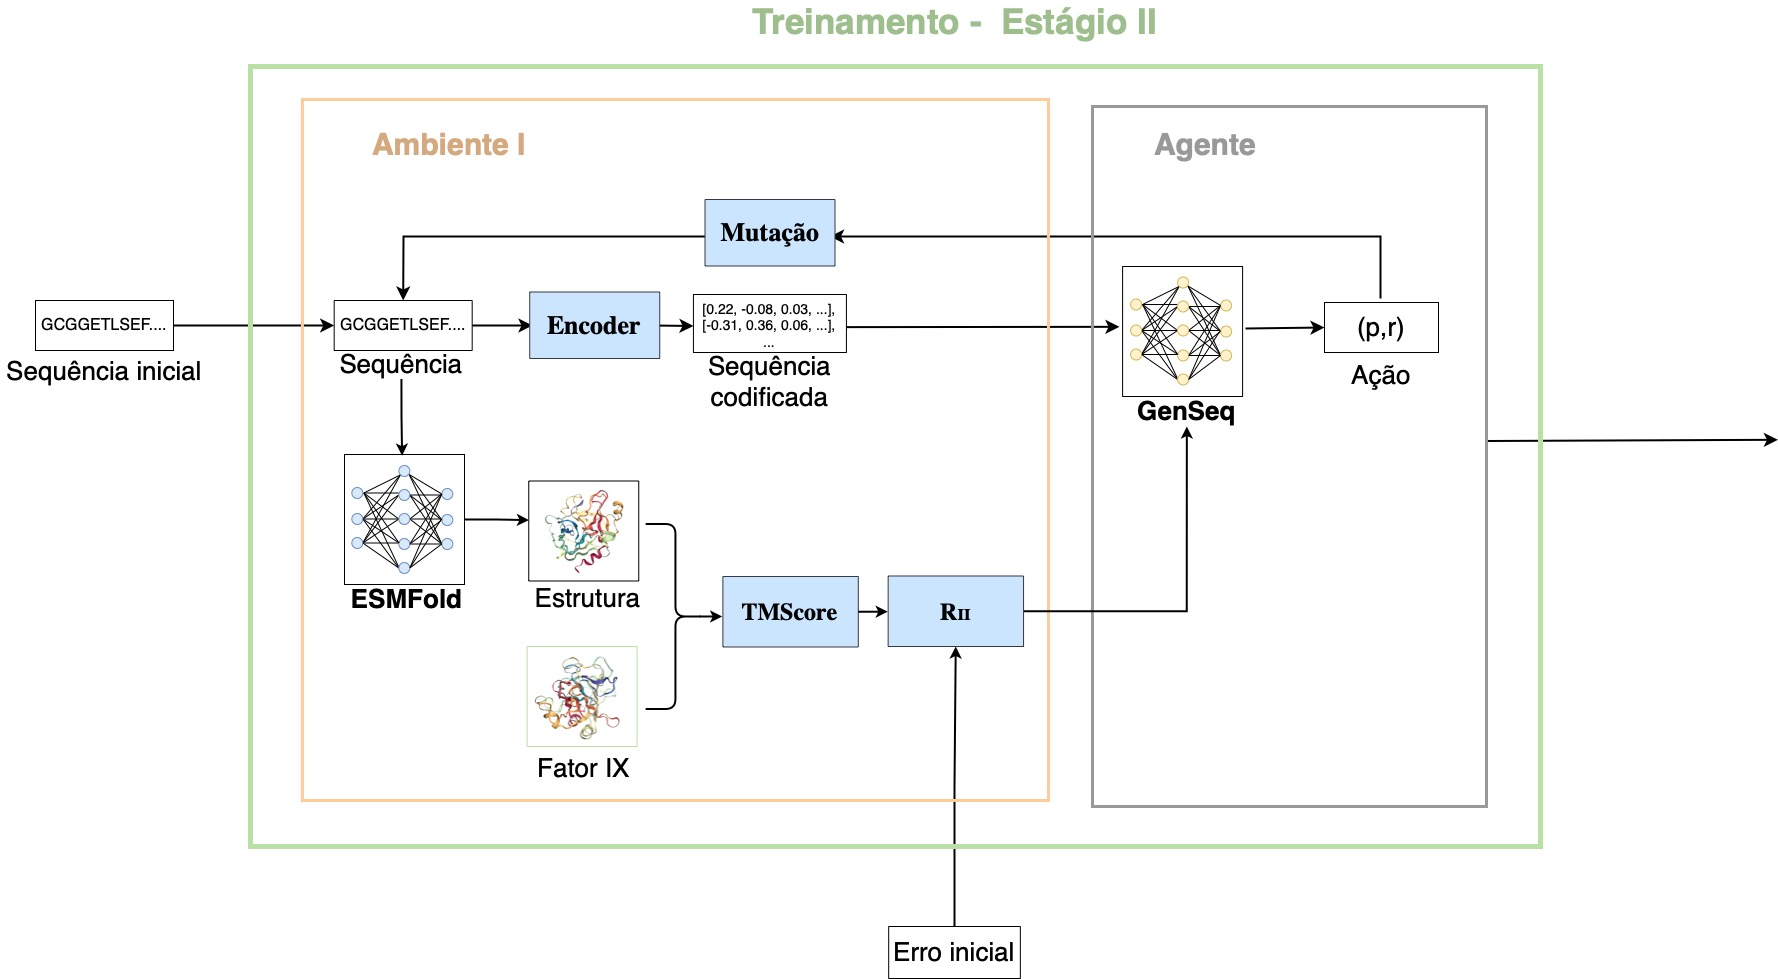
\includegraphics[width=.8\textwidth]{figuras/metodologia-Training.jpg}
  \caption{Segundo estágio - Treino}
\end{figure}

Neste estágio, o Agente foi treinado com um total de 60 mil de iterações, podendo executar até 45 mutações por episódio. 

\begin{table}[H]
  \centering
  \vspace{0.5cm}
  \begin{tabular}{r|lr}
  Parâmetro & Valor \\ 
  \hline                               % para uma linha horizontal
  Número máximo de mutações por episódio & 45 \\
  Erro mínimo no episódio & 0.05 \\
  Erro máximo no episódio & 0.083 \\
  Número de iterações & 60.000 \\
  a & 12 \\
  b & 200 \\
  c & 50 \\
  \end{tabular}
  \caption{Parâmetros preliminares}
  \end{table}

  Assim como no pré treino, a distribuição das recompensas do Agente ao longo do treinamento é 
  bem superior às recompensas de um Agente aleatório.  
  \begin{figure}[H]
    \centering
    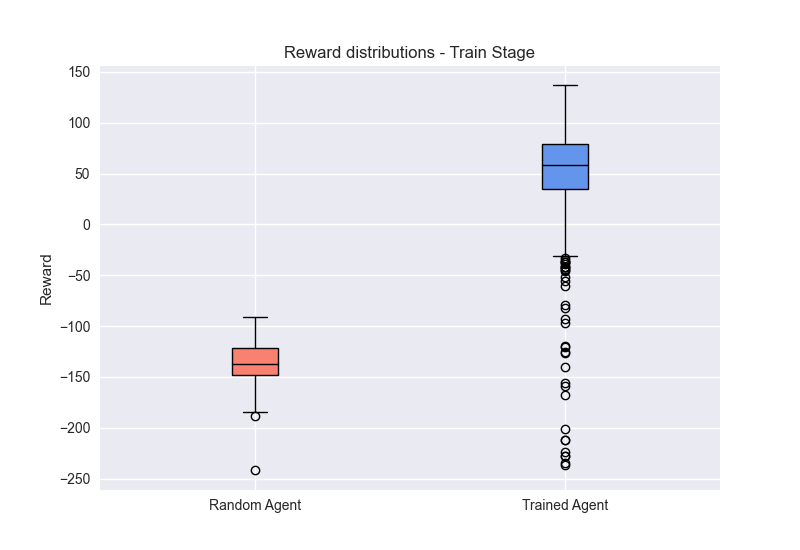
\includegraphics[width=.8\linewidth]{figuras/plot_box_train_reward.jpg}  
    \caption{Comparação do Agente treinado com um Agente aleatório}
    \label{fig:box-train}
  \end{figure}

  Repare que, devido ao pré treino, as recompensas médias do Agente são consideravelmente superiores
  à recompensa média do Agente aleatório desde os primeiros episódios. 
  \begin{figure}[H]
    \centering
    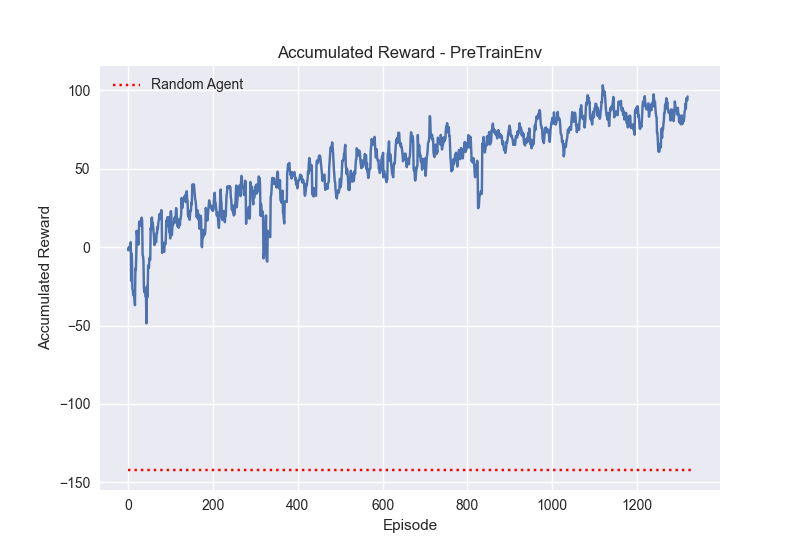
\includegraphics[width=.8\linewidth]{figuras/plot_train_reward.jpg}    
    \caption{Média móvel das recompensas por episódio - treino}
    \label{fig:rew_per_ep_train}
  \end{figure}
  

\section{Geração de sequências}
Por fim, o módulo de Geração de Sequências utiliza o agente treinado para gerar novas sequências que sejam capazes de mimetizar a estrutura alvo melhor do que a sequência inicial, em termos de \textit{TM-Score}.  
\begin{figure}[H]
  \centering
  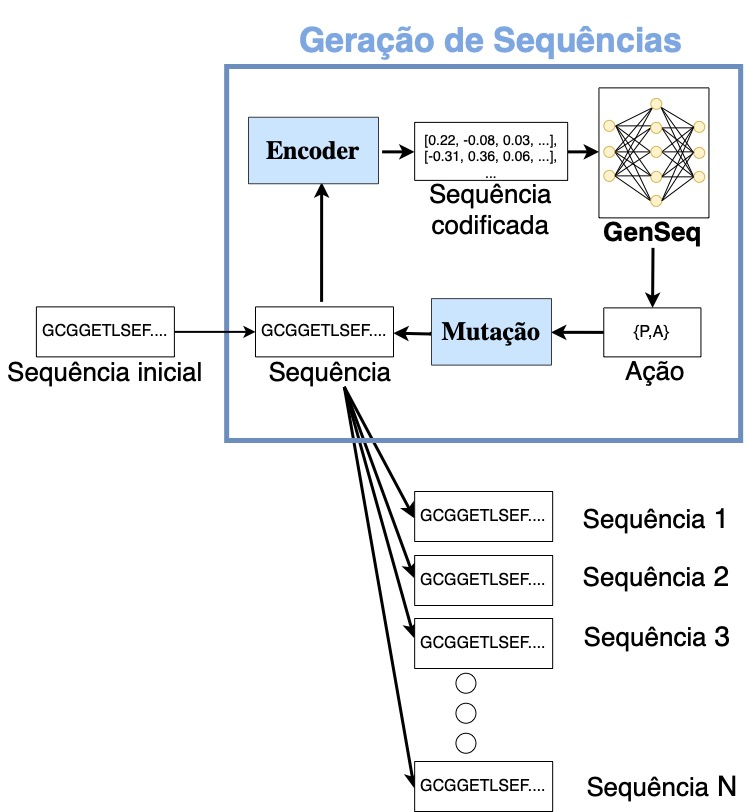
\includegraphics[width=.8\textwidth]{figuras/metodologia-Generating.jpg}
  \caption{Gerando sequência otimizada}
\end{figure}
